\section{处理器体系架构}

\subsection{Y86-64 指令集体系结构}

我们首先定义一个简单的指令集,作为我们处理器实现的运行示例。
因为受 x86-64 指令集的启发, 所以我们称我们的指令集为 Y86-64 指令集。
与 x86-64 相比, Y86-64 指令集的数据类型、指令和寻址方式都要少一些。
它的字节级编码也比较简单,机器代码没有相应的 x86-64 代码紧凑,不过设计它的 CPU 译码逻辑也要简单一些。
\begin{itemize}
    \item 寄存器: rax 、 rcx 、rdx 、 rbx 、rsp 、rbp 、rsi 、rdi 和 r8 到 r14 。
    \item 条件码: ZF(零标志)、SF(符号标志)、OF(溢出标志)
    \item 程序计数器:存放当前正在执行指令的地址。
    \item 状态码: AOK(正常)、 HLT(停止)、 ADR(地址错误)、 INS(无效指令)
    \item 内存:字节寻址的内存空间,小端法储存。
\end{itemize}

\subsubsection{Y86-64 指令}
\paragraph{指令编码}
\begin{figure}[H]
    \centering
    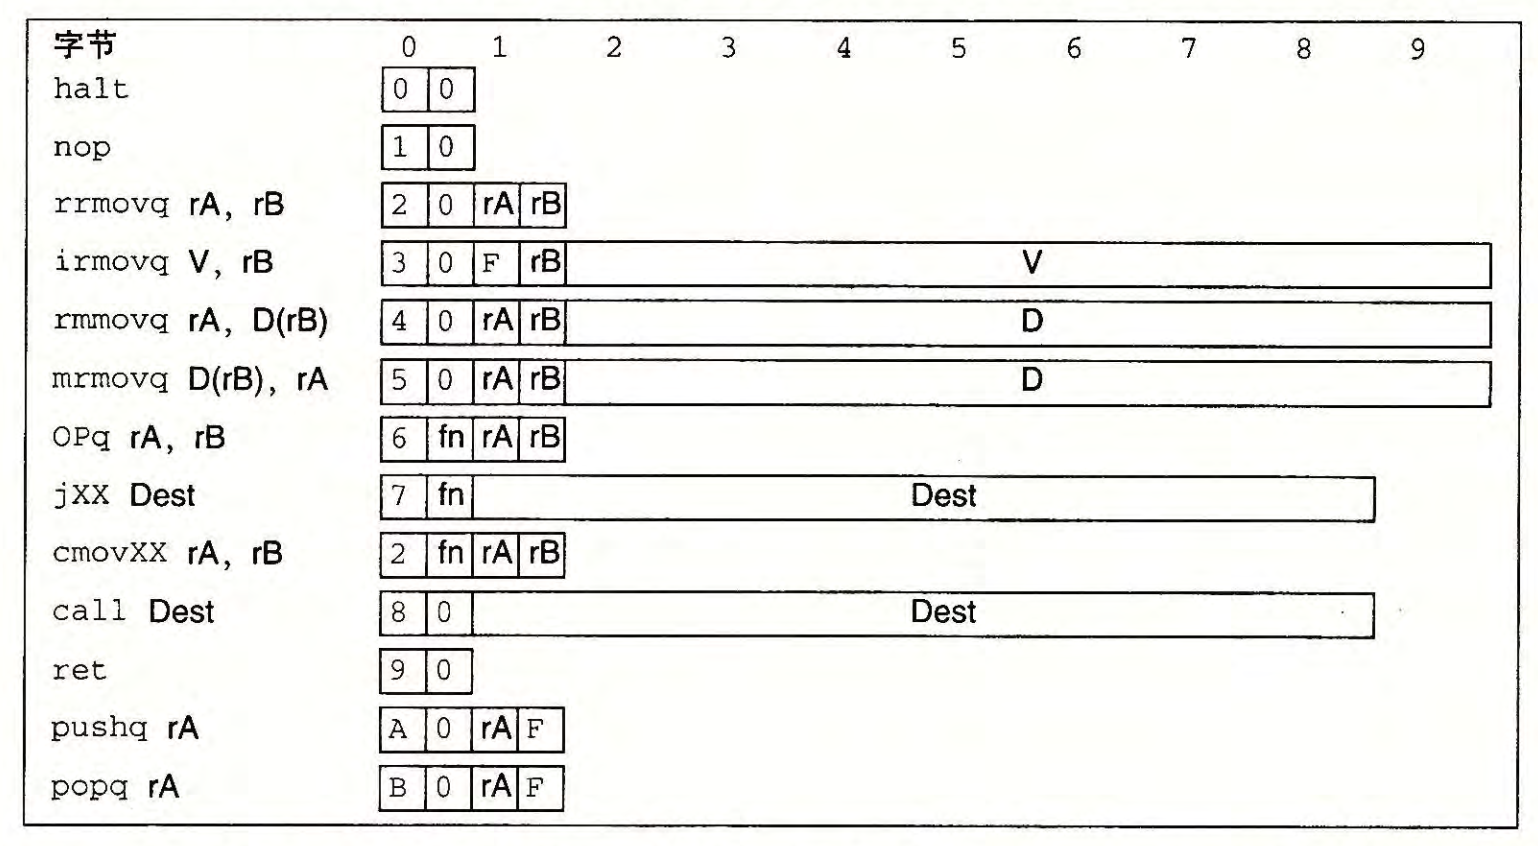
\includegraphics[width=0.8\textwidth]{instruction-encode.png}
\end{figure}
\begin{figure}[H]
    \centering
    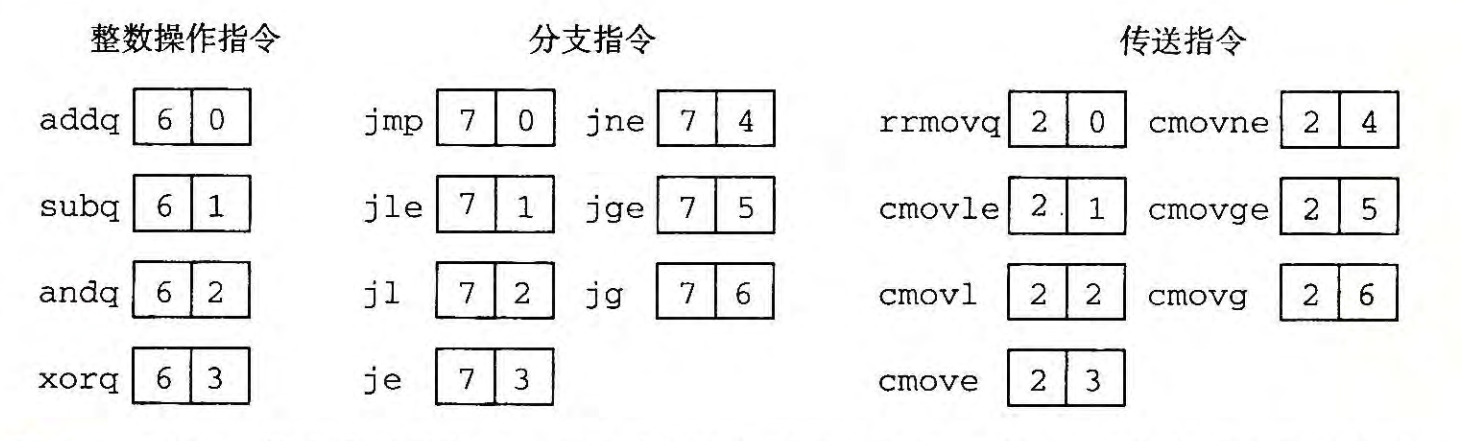
\includegraphics[width=0.8\textwidth]{instruction-function-encode.png}
\end{figure}

\begin{itemize}
    \item x86-64 的 movq 指令分成了 4 个不同的指令: irmovq 、 rrmovq 、 mrmovq 和 rmmovq 。分别显式地指明源和目的的格式。
    \item 内存引用方式是简单的基址和偏移量形式。在地址计算中,不支持第二变址寄存器 (second index register) 和任何寄存器值的伸缩 (scaling)。
    \item 4 个整数操作指令 (OPq) : addq 、 subq 、 andq 和 xorq 。 它们只对寄存器数据进行操作,会设置 3 个条件码 ZF 、 SF 和 OF 。
    \item 7 个跳转指令 (jXX) : jmp 、 jle 、 jl 、 je 、 jne 、 jge 和 jg 。 它们根据条件码的值来决定是否跳转。
    \item 有 6 个条件传送指令 (cmovXX) : cmovle 、 cmovl 、 cmove 、 cmovne 、 cmovge 和 cmovg 。 它们根据条件码的值来决定是否执行传送操作。
    \item call 指令将返回地址入栈,然后跳到目的地址。 ret 指令从这样的调用中返回。
    \item pushq 和 popq 指令实现了入栈和出栈操作。
    \item halt 指令停止指令的执行。
    \item nop 指令什么也不做,只是简单地前进到下一条指令。
\end{itemize}

每条指令需要 1~10 个字节不等,这取决于需要哪些字段。每条指令的第一个字节表明指令的类型。这个字节分为两个部分,每部分 4 位:高 4 位是代码 (code) 部分,低 4 位是功能 (function) 部分。

\paragraph{寄存器编码}
\begin{figure}[H]
    \centering
    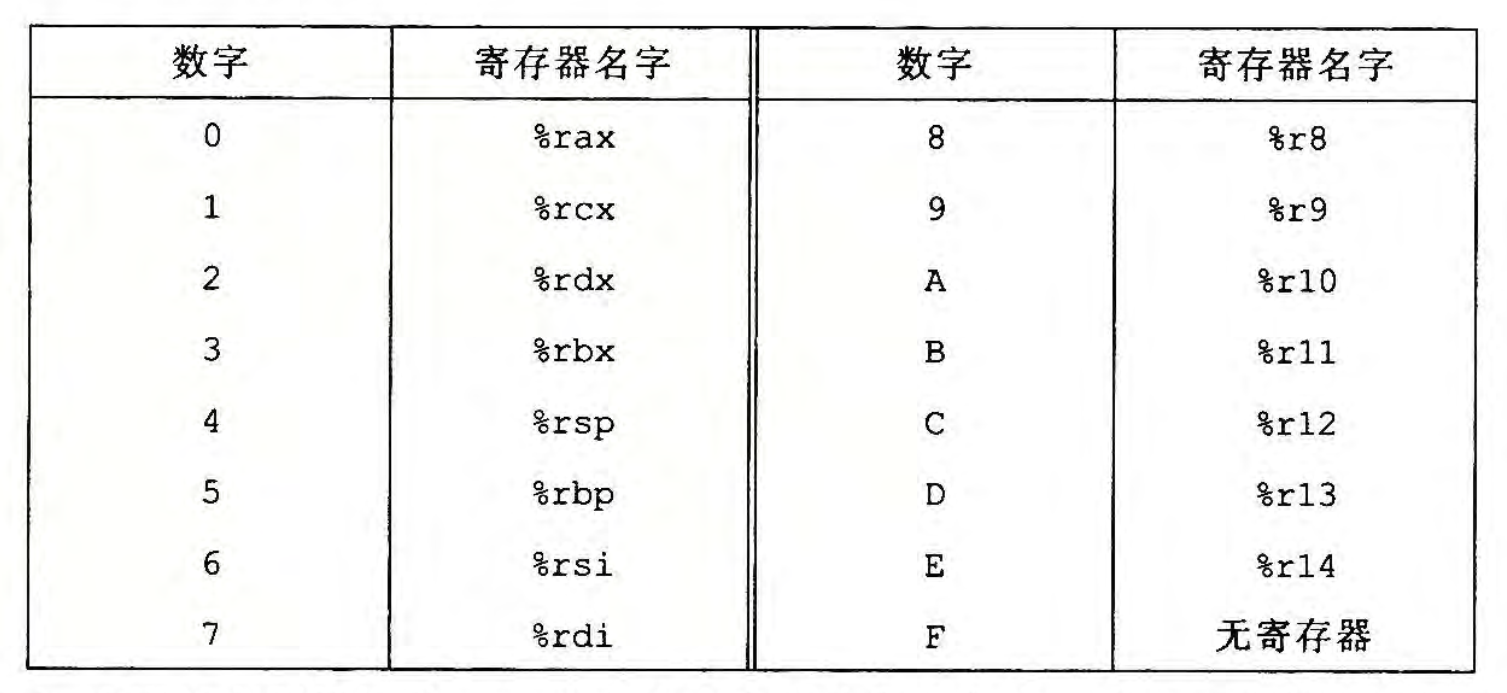
\includegraphics[width=0.8\textwidth]{register-encode.png}
\end{figure}

15 个程序寄存器中每个都有一个相对应的范围在 0 到 OxE 之间的寄存器标识符 (register ID) 。 当需要指明不应访问任何寄存器时,就用 ID 值 OxF 来表示。

\subsubsection{Y86-64 异常}

\begin{figure}[H]
    \centering
    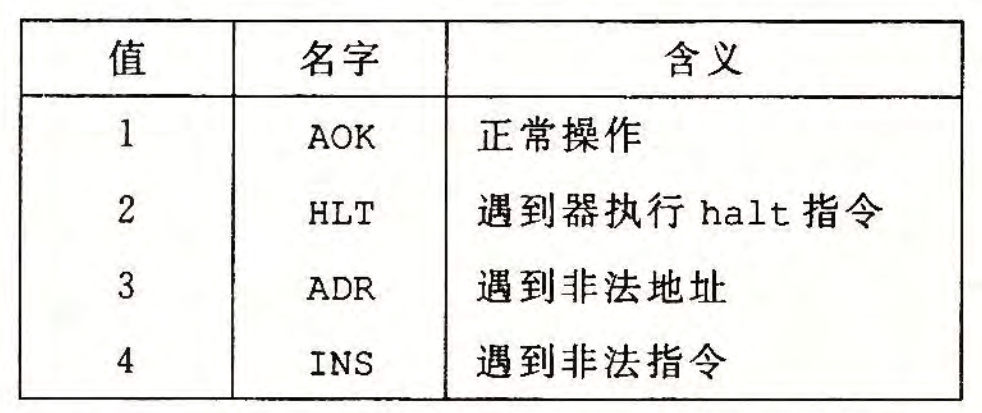
\includegraphics[width=0.6\textwidth]{status-code.png}
\end{figure}

Y86-64 中的状态码描述程序执行的总体状态。正常执行时,状态码为 AOK 。当程序执行 halt 指令时,状态码变为 HLT 。如果程序试图访问无效的内存地址,状态码变为 ADR 。如果程序试图执行无效指令,状态码变为 INS 。
对于 Y86-64, 当遇到这些异常的时候,我们就简单地让处理器停止执行指令。在更完整的设计中,处理器通常会调用一个异常处理程序(exception handler), 这个过程被指定用来处理遇到的某种类型的异常。

\subsubsection{Y86-64 程序}
\begin{lstlisting}[style=ASMStyle]
; Execution begins at address 0
        .pos 0
        irmovq stack, %rsp      ; Set up stack pointer
        call main               ; Execute main program
        halt                    ; Terminate program

; Array of 4 elements
array:  .align 8
        .quad 0x000d000d000d
        .quad 0x00c000c000c0
        .quad 0x0b000b000b00
        .quad 0xa000a000a000

main:
        irmovq array, %rdi
        irmovq $4, %rsi
        call sum                ; sum(array, 4)
        ret

; long sum(long *start, long count)
; start in %rdi, count in %rsi
sum:
        irmovq $8, %r8          ; Constant 8
        irmovq $1, %r9          ; Constant 1
        xorq %rax, %rax         ; sum = 0
        andq %rsi, %rsi         ; Set CC
        jmp     test            ; Goto test
loop:
        mrmovq (%rdi), %r10     ; Get *start
        addq %r10, %rax         ; Add to sum
        addq %r8, %rdi          ; start++
test:
        subq %r9, %rsi          ; count--. Set CC
        jne     loop            ; Stop when 0
        ret                     ; Return

; Stack starts here and grows to lower addresses
        .pos 0x200
stack:
\end{lstlisting}

注意到:
\begin{itemize}
    \item 由于 Y86-64 是一个简化的指令集,所以相较于 x86-64, Y86-64 的汇编代码会更加复杂。
    \item 程序从地址 0 处开始。
    \item 初始化栈指针,指明地址 0x200 处是栈的起始位置,低地址增长。须保证栈不会增长得太大以至千覆盖了代码或者其他程序数据。
\end{itemize}

\begin{sidenote}{两个特别的指令}
    在 Y86-64 和 x86-64 中:
    \begin{itemize}
        \item pushq \%rsp 会压入 \%rsp 的原始值。
        \item popq \%rsp 会将 \%rsp 置为从内存中读出的值。
    \end{itemize}
\end{sidenote}

\subsection{逻辑设计}

\subsubsection{逻辑门}
逻辑门是数字电路的基本计算单元。它们产生的输出,等于它们输入位值的某个布尔函数。
辑门总是活动的,一旦一个门的输入变化了,在很短的时间内,输出就会相应地变化。
\begin{figure}[H]
    \centering
    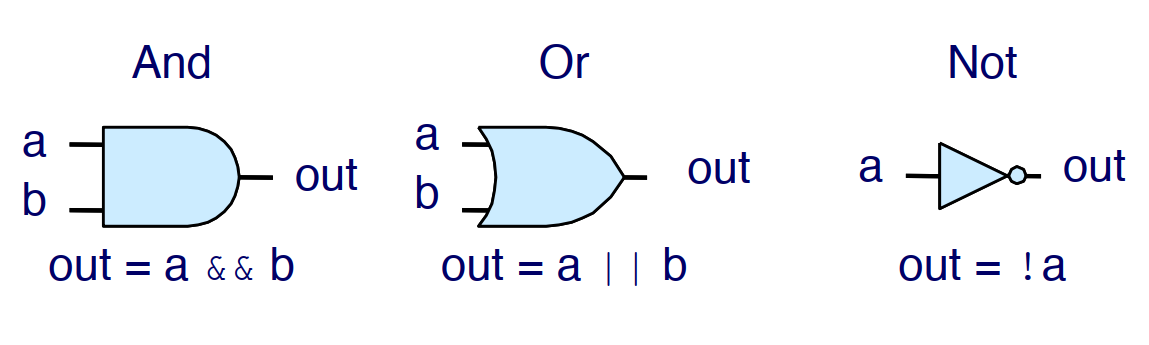
\includegraphics[width=0.8\textwidth]{logic-gate.png}
\end{figure}
\subsubsection{组合电路}

将很多的逻辑门组合成一个网,就能构建计算块,称为组合电路。

\paragraph{位相等电路}

位相等电路有两个输入 a 和 b ,有唯一的输出 eq, 当 a 和 b 都是 1 或都是 0 时,输出为 1 。

\begin{figure}[H]
    \centering
    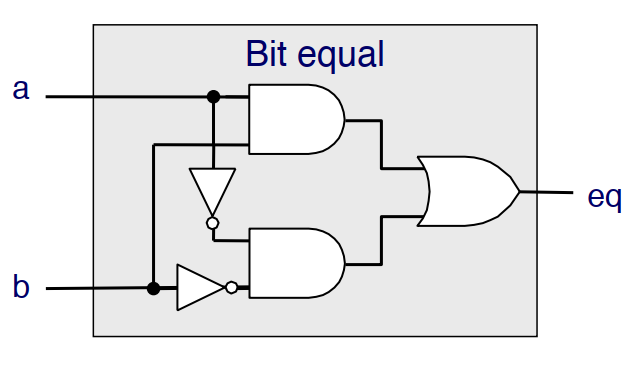
\includegraphics[width=0.8\textwidth]{bit-equality.png}
\end{figure}
\begin{lstlisting}[style=CStyle]
bool eq = (a && b) || (!a && !b);
\end{lstlisting}

\paragraph{多路复用器}
多路复用器根据输入控制信号的值,从一组不同的数据信号中选出一个。
在这个单个位的多路复用器中,两个数据信号是输入位 a 和 b ,控制信号是输入位 s 。
当 s 为 1 时,输出等于 a ;而当 s 为 0 时,输出等于 b 。

\begin{figure}[H]
    \centering
    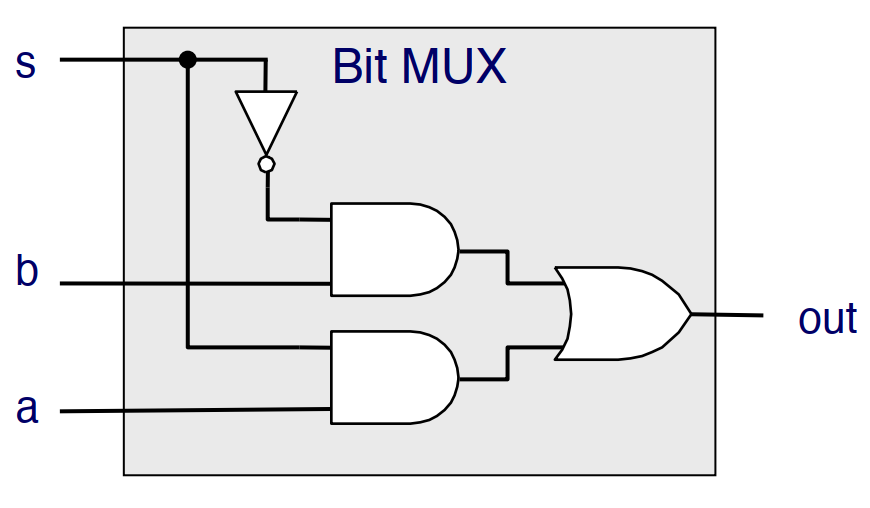
\includegraphics[width=0.8\textwidth]{bit-multiplexor.png}
\end{figure}
\begin{lstlisting}[style=CStyle]
bool out = (s && a) || (!s && b);
\end{lstlisting}

\subsubsection{字级的组合电路}

通过将逻辑门组合成大的网,可以构造出能计算更加复杂函数的组合电路。

\paragraph{字相等电路}

字相等电路当且仅当 A 的每一位都和 B 的相应位相等时,输出才为 1 。

\begin{figure}[H]
    \centering
    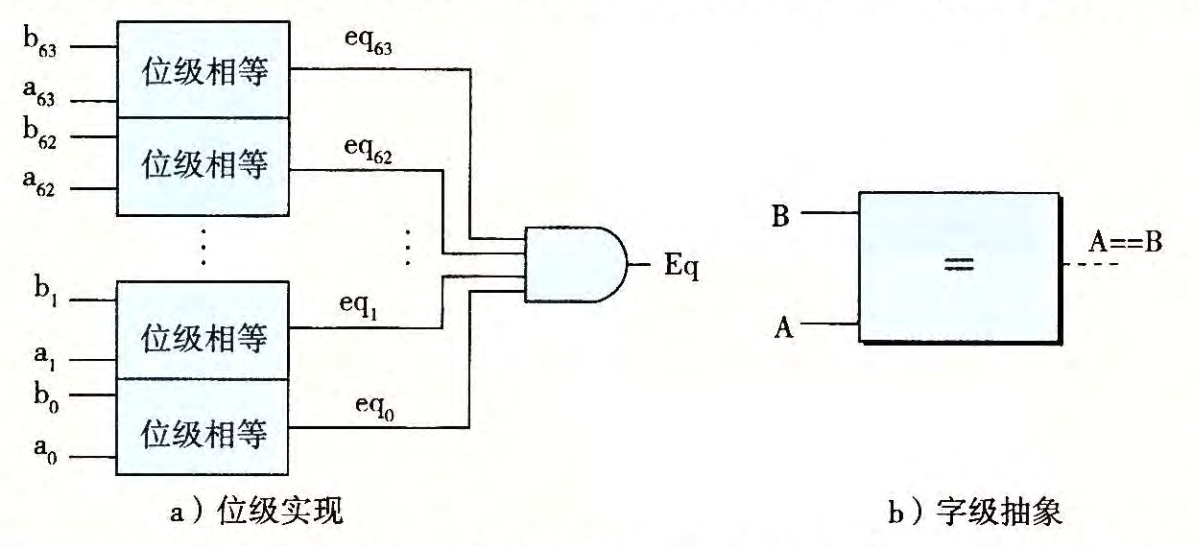
\includegraphics[width=0.8\textwidth]{word-equality.png}
\end{figure}
\begin{lstlisting}[style=CStyle]
bool Eq = (A == B);
\end{lstlisting}

\paragraph{字级的多路复用器电路}

字级的多路复用器电路根据控制输入位 s , 产生一个 64 位的字 Out ,等于两个输入字 A 或者 B 中的一个。
处理器中会用到很多种多路复用器,使得我们能根据某些控制条件,从许多源中选出一个字。
在 HCL 中,多路复用函数是用情况表达式来描述的。
情况表达式的通用格式如下:
\begin{lstlisting}[style=CStyle]
[
    select1 : expr1;
    select2 : expr2;
    .
    .
    .
    selectk : exprk;
]
\end{lstlisting}

我们不要求不同的选择表达式之间互斥。
从逻辑上讲,这些选择表达式是顺序求值的,且第一个求值为 1 的情况会被选中。
\begin{figure}[H]
    \centering
    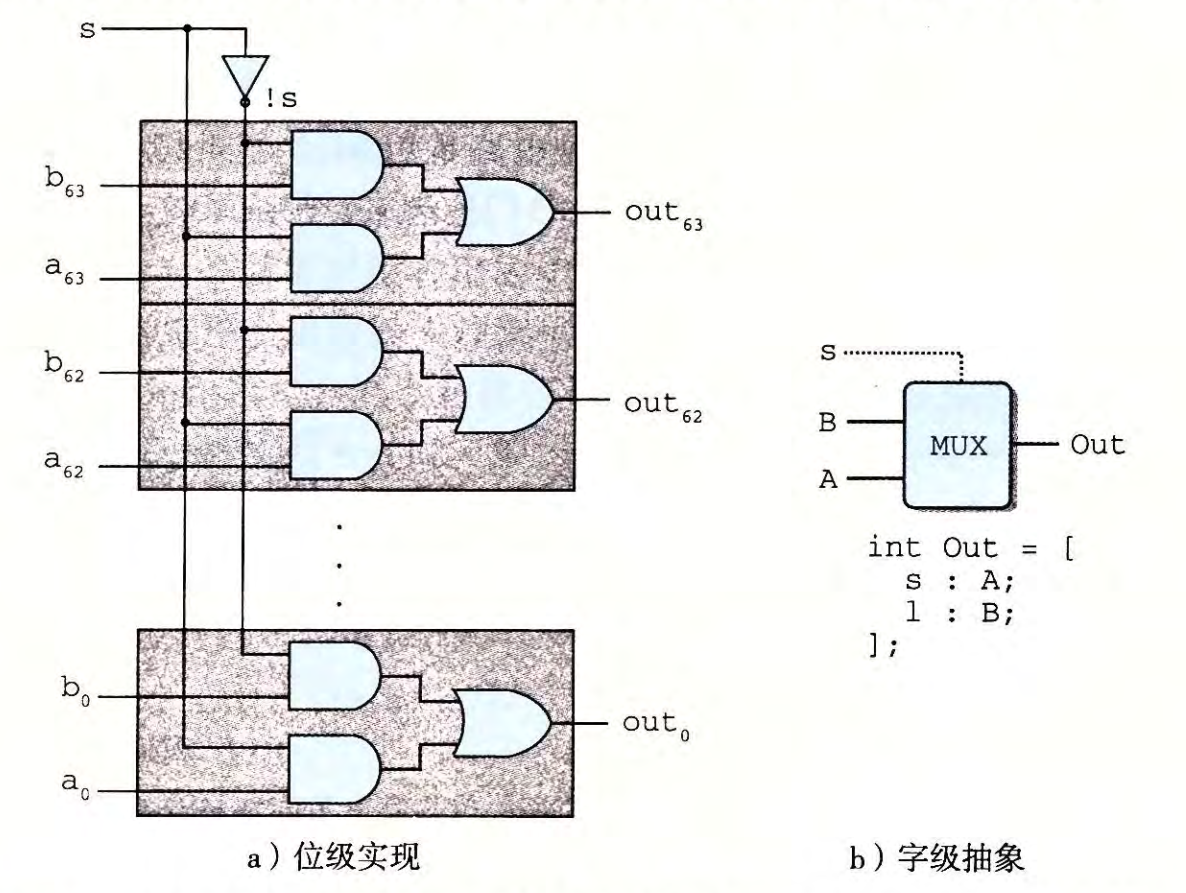
\includegraphics[width=0.8\textwidth]{word-multiplexor.png}
\end{figure}
\begin{lstlisting}[style=CStyle]
word Out = [
    s: A;
    1: B;
] ;
\end{lstlisting}
\begin{figure}[H]
    \centering
    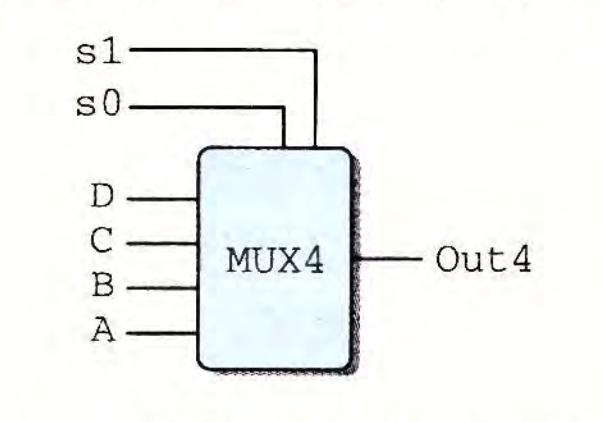
\includegraphics[width=0.6\textwidth]{4-way-multiplexor.png}
\end{figure}
\begin{lstlisting}[style=CStyle]
word Out4 = [
    !s1 && !s0 : A; # 00
    !s1        : B; # 01
    !s0        : C; # 10
    1          : D; # 11
];
\end{lstlisting}
\begin{figure}[H]
    \centering
    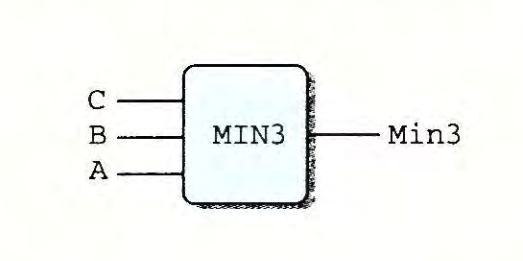
\includegraphics[width=0.6\textwidth]{min-multiplexor.png}
\end{figure}
\begin{lstlisting}[style=CStyle]
word Min3 = [
    A <= B && A <= C : A;
    B <= A && B <= C : B;
    1                : C;
];
\end{lstlisting}

\paragraph{算术逻辑单元}

算术逻辑单元 (ALU) 是一种很重要的组合电路。
有标号为 A 和 B 的两个数据输入,以及一个控制输入。
根据控制输入的设置,电路会对数据输入执行不同的算术或逻辑操作。

\begin{figure}[H]
    \centering
    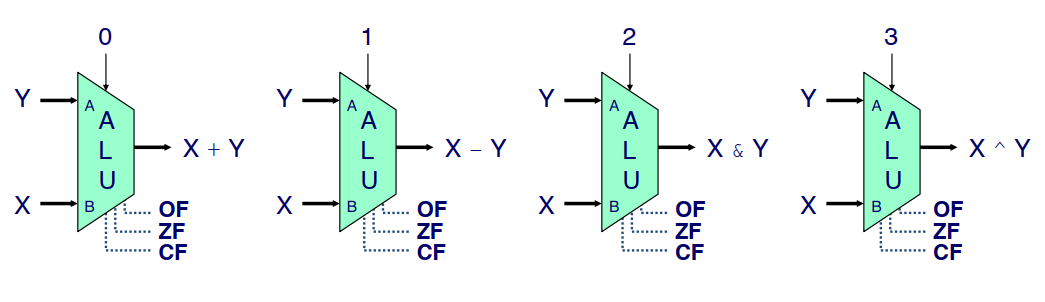
\includegraphics[width=0.8\textwidth]{ALU.png}
\end{figure}


\subsubsection{存储器}
组合电路从本质上讲,不存储任何信息。为了产生时序电路,我们必须引入按位存储信息的设备。
存储设备都是由同一个时钟控制的,时钟是一个周期性信号,决定什么时候要把新值加载到设备中。
有两类存储器设备:
\begin{itemize}
    \item 时钟寄存器(简称寄存器):存储单个位或字。时钟信号控制寄存器加载输入值。
    \item 随机访问存储器(简称内存):存储多个字,用地址来选择该读或该写哪个字。
          \begin{itemize}
              \item 处理器的虚拟内存系统:硬件和操作系统软件结合起来使处理器可以在一个很大的地址空间内访问任意的字。
              \item 寄存器文件:用于存储处理器操作数的小型、快速的存储单元集,寄存器标识符作为地址。
          \end{itemize}
\end{itemize}

\paragraph{寄存器}
大多数时候,寄存器都保待在稳定状态(用 x 表示),产生的输出等千它的当前状态。
信号沿着寄存器前面的组合逻辑传播,这时,产生了一个新的寄存器输入(用 y 表示),但只要时钟是低电位的,寄存器的输出就仍然保持不变。
当时钟变成高电位的时候,输入信号就加载到寄存器中,成为下一个状态 y , 直到下一个时钟上升沿,这个状态就一直是寄存器的新输出。
\begin{figure}[H]
    \centering
    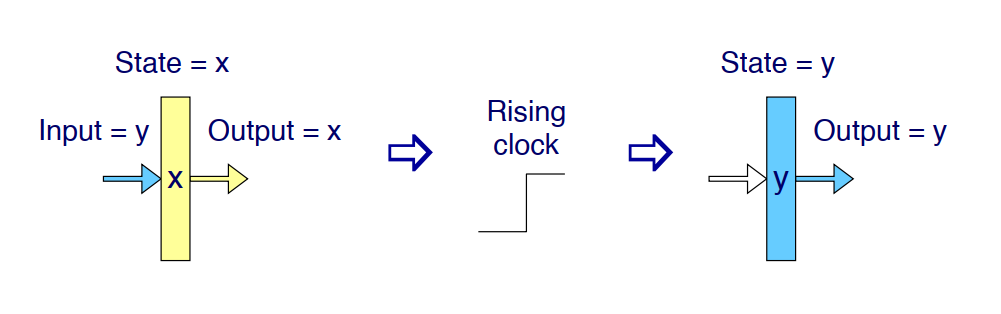
\includegraphics[width=0.8\textwidth]{register.png}
\end{figure}
\begin{figure}[H]
    \centering
    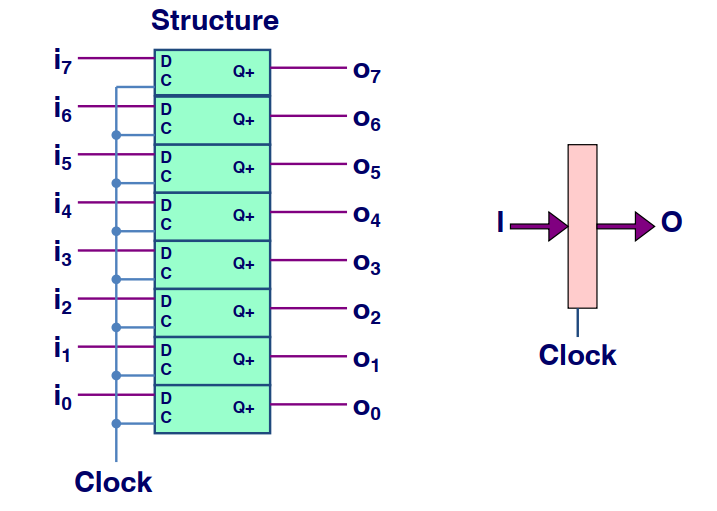
\includegraphics[width=0.8\textwidth]{registers.png}
\end{figure}

\paragraph{寄存器文件}
寄存器文件有两个读端口 (A 和 B) ,还有一个写端口 (W) 。这样一个多端口随机访问存储器允许同时进行多个读和写操作。

当 srcA 或 srcB 被设成某个寄存器 ID 时,在一段延迟之后,存储在相应程序寄存器的值就会出现在 valA 或 valB 上。

向寄存器文件写入字是由时钟信号控制的,控制方式类似于将值加载到时钟寄存器。
每次时钟上升时,输入 valW 上的值会被写入输入 dstW 上的寄存器 ID 指示的程序寄存器。
当 dstW 设为特殊的 ID 值 0xF 时,不会写任何程序寄存器。
\begin{figure}[H]
    \centering
    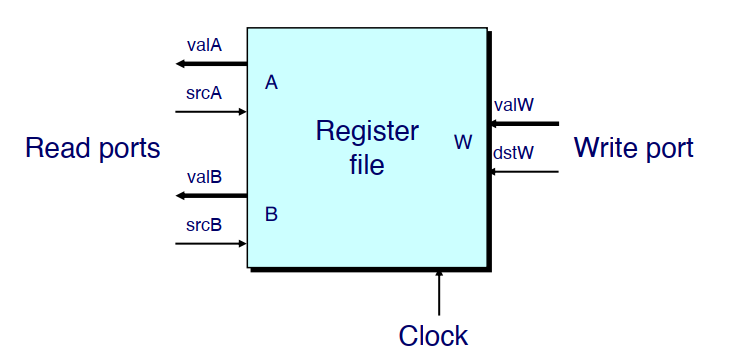
\includegraphics[width=0.8\textwidth]{register-file.png}
\end{figure}

\paragraph{内存}

内存有一个地址输入,一个写的数据输入,以及一个读的数据输出。

同寄存器文件一样,从内存中读的操作方式类似于组合逻辑:如果我们在输入 address 上提供一个地址,
并将 write 控制信号设置为 0, 那么在经过一些延迟之后,存储在那个地址上的值会出现在
输出 data 上。如果地址超出了范围, error 信号会设置为 1, 否则就设置为 0 。

写内存是由时钟控制的:我们将 address 设置为期望的地址,将 data in 设置为期望的值,而 write 设
置为 1 。然后当我们控制时钟时,只要地址是合法的,就会更新内存中指定的位置。
\begin{figure}[H]
    \centering
    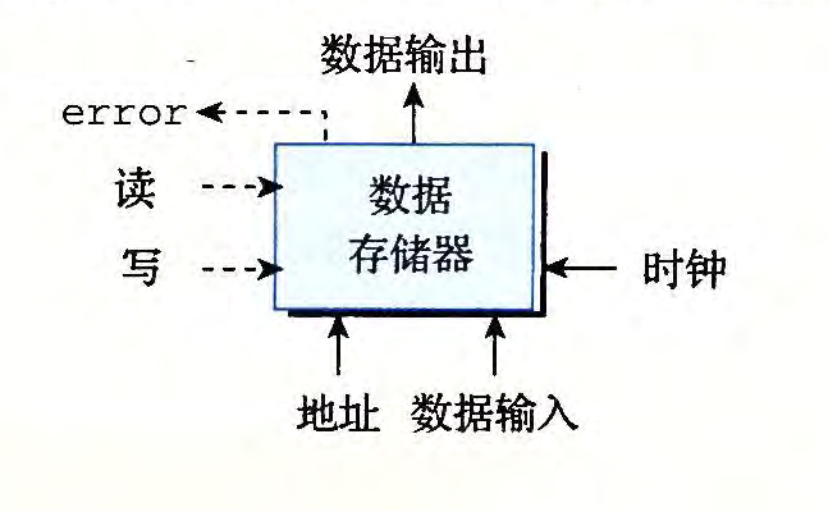
\includegraphics[width=0.6\textwidth]{random-access-memory.png}
\end{figure}

\subsection{Y86-64 的顺序实现}

通常,处理一条指令包括很多操作。将它们组织成某个特殊的阶段序列,即使指令的动作差异很大,但所有的指令都遵循统一的序列。
创建这样一个框架,我们就能够设计一个充分利用硬件的处理器。
\begin{itemize}
    \item 取指 (fetch):
          将程序计数器寄存器作为地址,读取指令的字节。 PC 增加器 (PC incrementer) 计算 valP ,即增加了的程序计数器 。
    \item 译码 (decode):
          寄存器文件有两个读端口 A 和 B ,从这两个端口同时读寄存器值 valA 和 valB 。
    \item 执行 (execute):
          执行阶段会根据指令的类型,将 ALU 用于不同的目的。
          对整数操作,它要执行指令所指定的运算。
          对其他指令,它会作为一个加法器来计算增加或减少栈指针,或者计算有效地址,或者只是简单地加 0 ,将一个输入传递到输出。

          条件码寄存器 (CC) 有三个条件码位。 ALU 负责计算条件码的新值。
          当执行条件传送指令时,根据条件码和传送条件来计算决定是否更新目标寄存器。
          同样,当执行一条跳转指令时,会根据条件码和跳转类型来计算分支信号 Cnd 。
    \item 访存 (memory):
          在执行访存操作时,数据内存读出或写入一个内存字。
    \item 写回 (write back):
          寄存器文件有两个写端口。端口 E 用来写 ALU 计算出来的值,而端口 M 用来写从数据内存中读出的值。
    \item 更新 PC (PC update):
          程序计数器的新值选择自:下一条指令的地址 valP ;调用指令或跳转指令指定的目标地址 valE ;从内存读取的返回地址 valM 。
\end{itemize}
\begin{figure}[H]
    \centering
    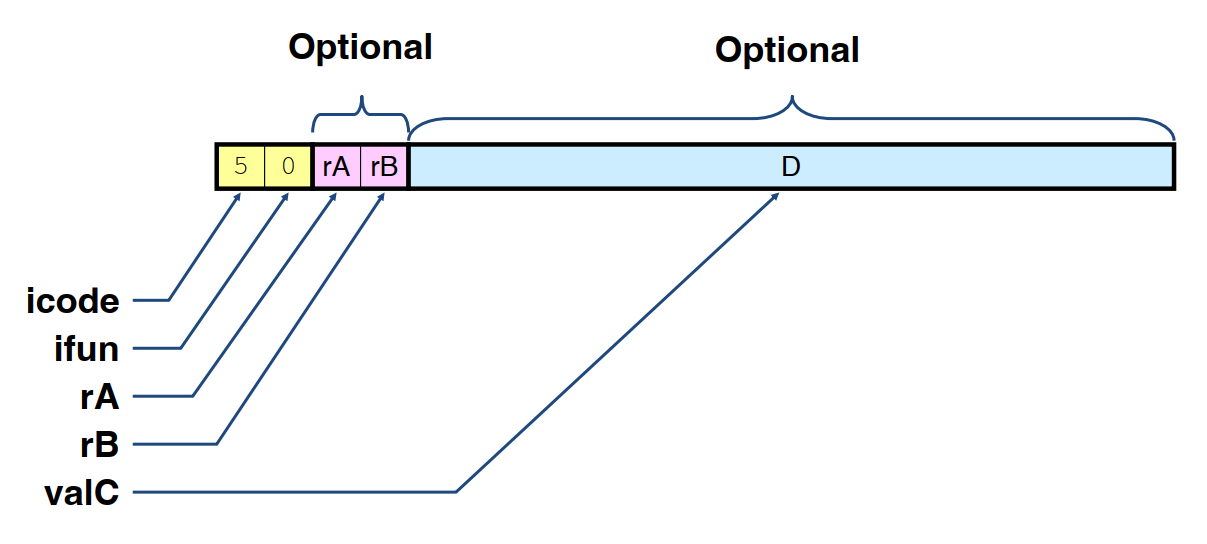
\includegraphics[width=0.8\textwidth]{instruction-decode.png}
\end{figure}
\begin{figure}[H]
    \centering
    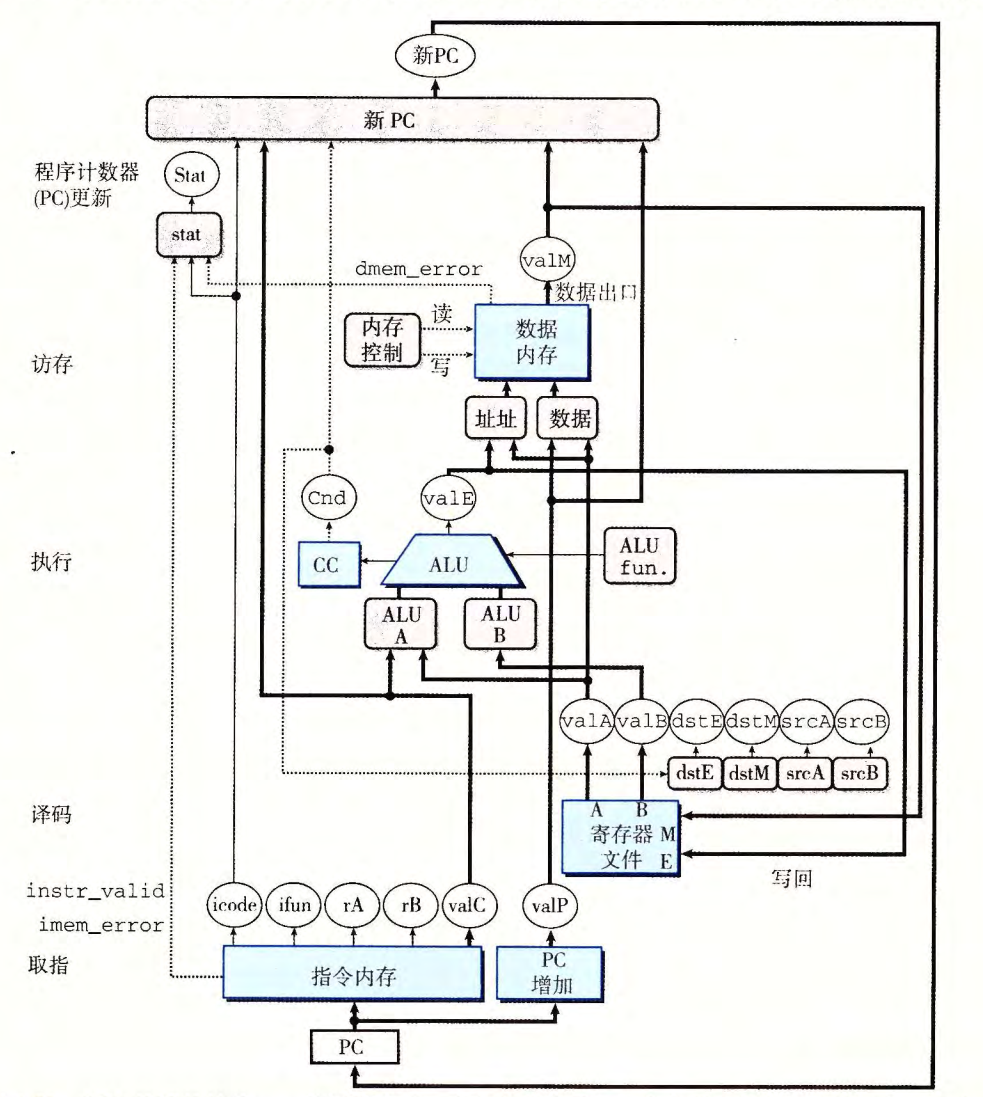
\includegraphics[width=0.8\textwidth]{SEQ-structure.png}
\end{figure}
\begin{figure}[H]
    \centering
    \begin{subfigure}[t]{0.5\textwidth}
        \centering
        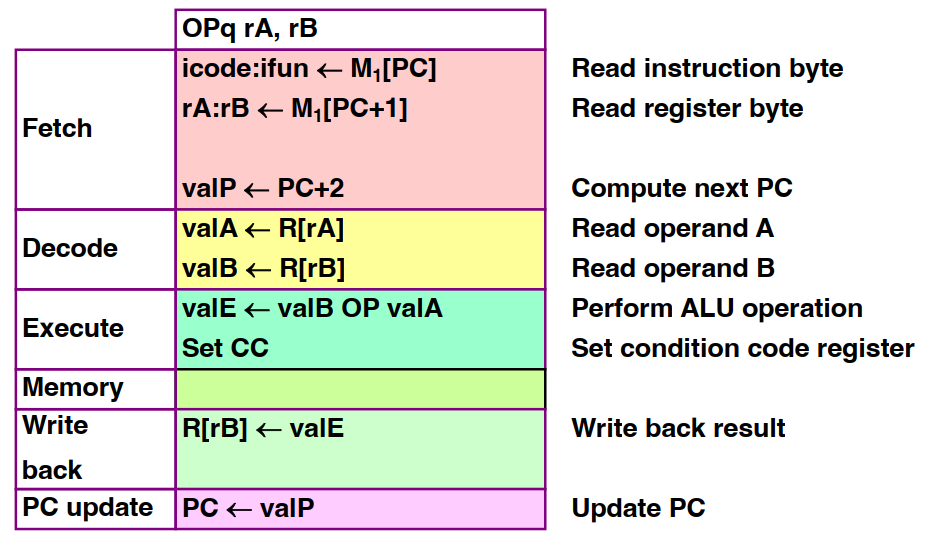
\includegraphics[width=\linewidth]{ops-stage-computation.png}
    \end{subfigure}\hfill
    \begin{subfigure}[t]{0.5\textwidth}
        \centering
        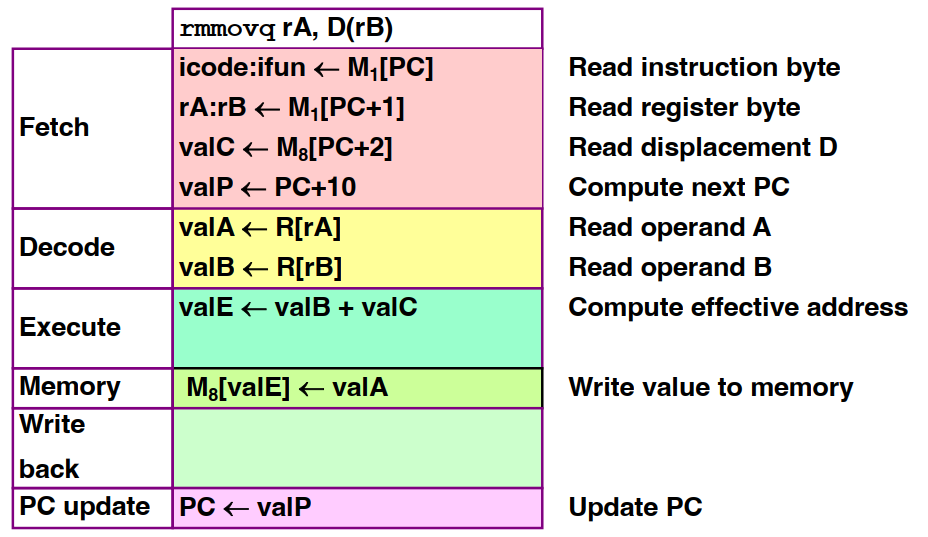
\includegraphics[width=\linewidth]{rmmovq-stage-computation.png}
    \end{subfigure}
    \medskip
    \begin{subfigure}[t]{0.5\textwidth}
        \centering
        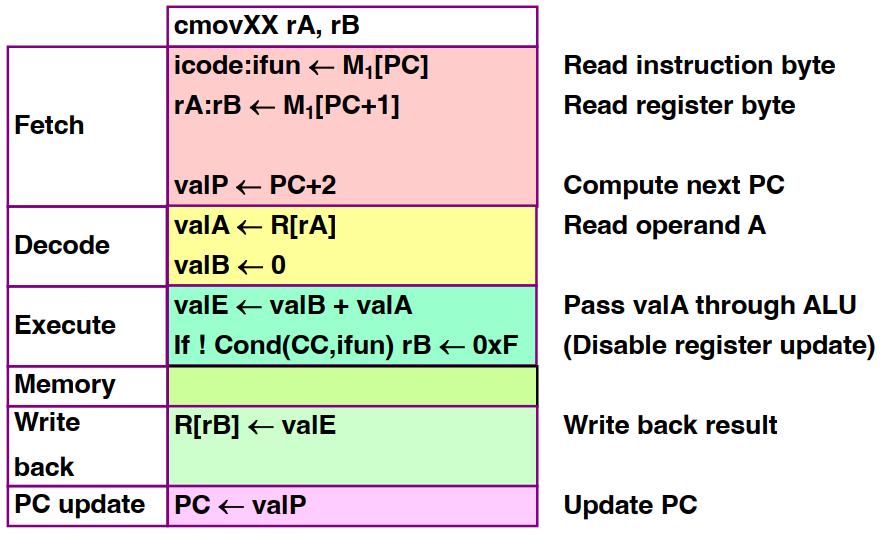
\includegraphics[width=\linewidth]{cmov-stage-computation.png}
    \end{subfigure}\hfill
    \begin{subfigure}[t]{0.5\textwidth}
        \centering
        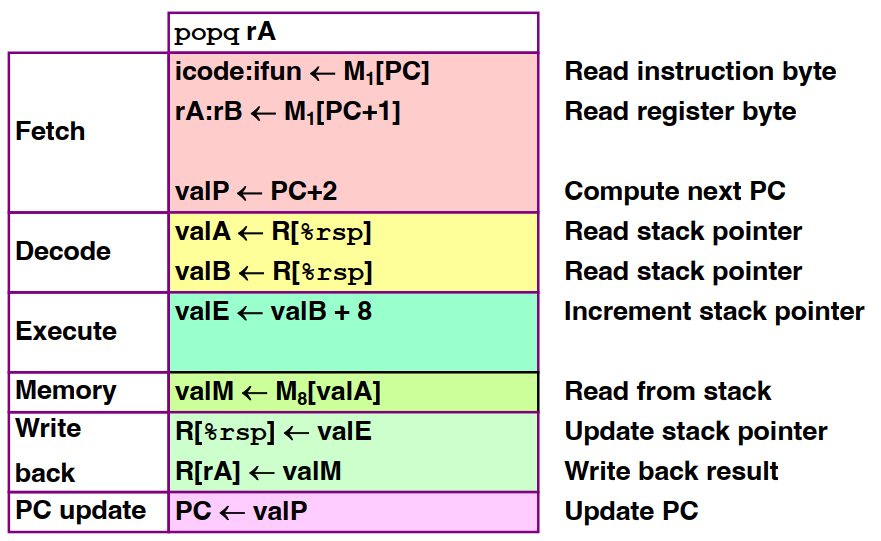
\includegraphics[width=\linewidth]{popq-stage-computation.png}
    \end{subfigure}
    \medskip
    \begin{subfigure}[t]{0.5\textwidth}
        \centering
        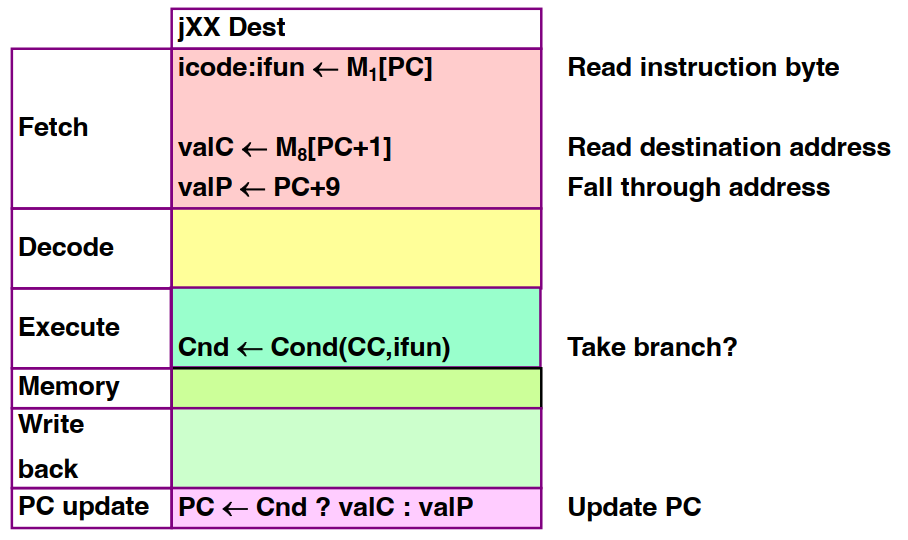
\includegraphics[width=\linewidth]{jmp-stage-computation.png}
    \end{subfigure}\hfill
    \begin{subfigure}[t]{0.5\textwidth}
        \centering
        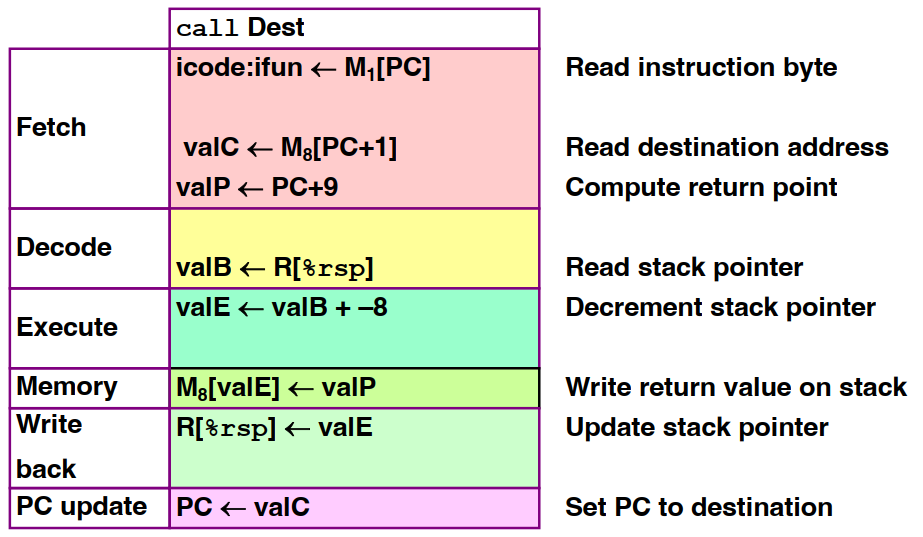
\includegraphics[width=\linewidth]{call-stage-computation.png}
    \end{subfigure}
    \medskip
    \begin{subfigure}[t]{0.5\textwidth}
        \centering
        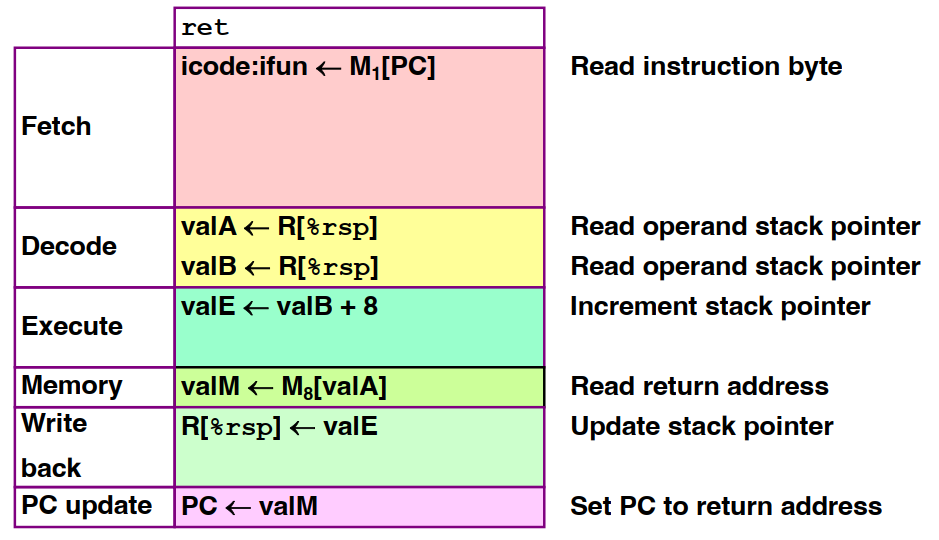
\includegraphics[width=\linewidth]{ret-stage-computation.png}
    \end{subfigure}
\end{figure}

\subsubsection{取指阶段}

\begin{figure}[H]
    \centering
    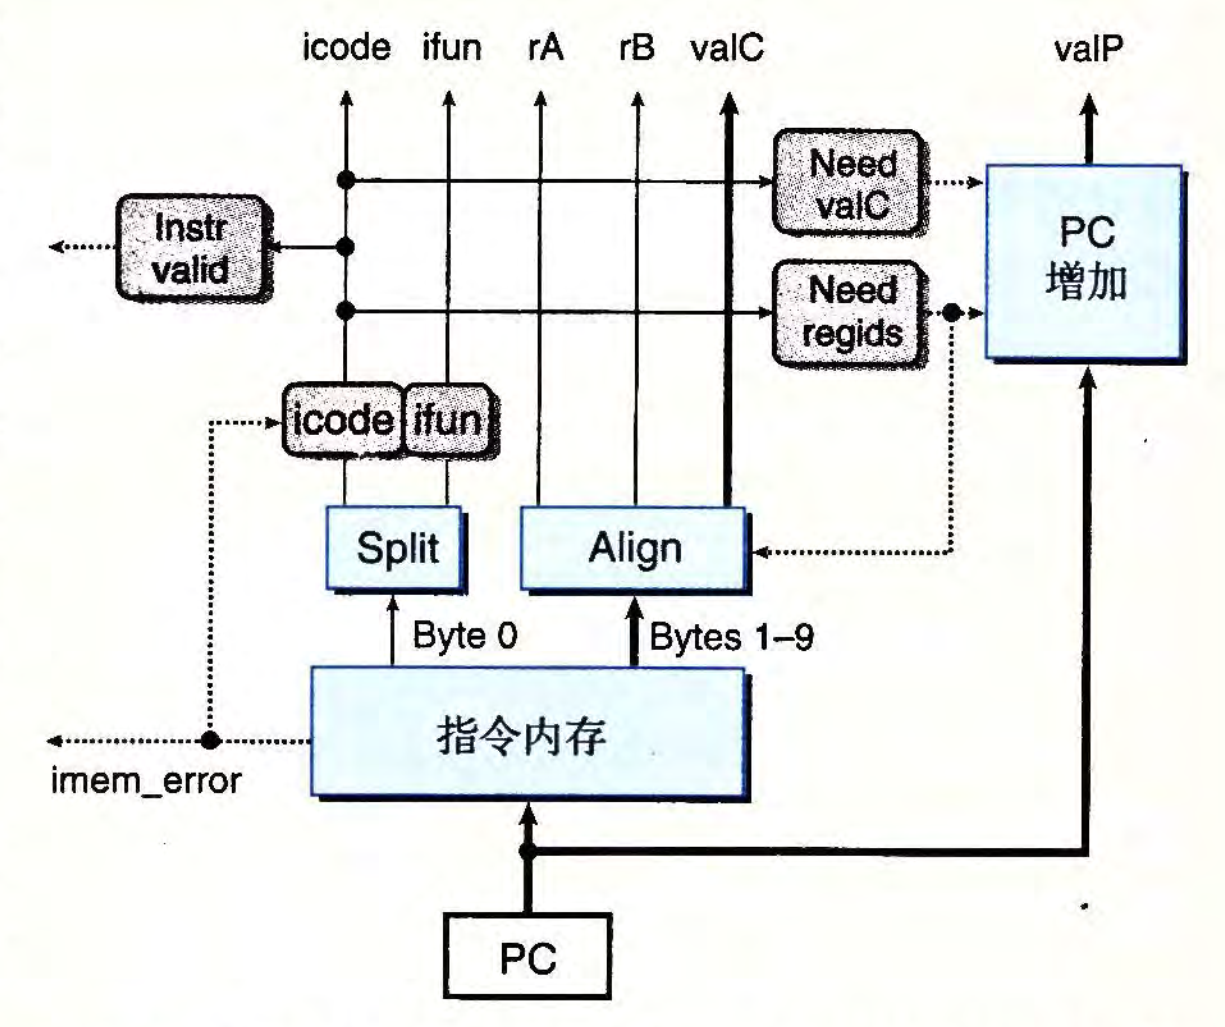
\includegraphics[width=0.5\textwidth]{fetch.png}
\end{figure}

以 PC 作为第一个字节(字节 0 )的地址,这个单元一次从内存读出 10 个字节。
第一个字节被解释成指令字节,标号为 "Split" 的单元)分为两个 4 位的数。
然后,标号为 "icode" 和 "ifun" 的控制逻辑块计算指令和功能码,或者使之等于从内存读出的值,或者当指令地址不合法时(由信号 imem error 指明),使这些值对应于 nop 指令。
根据使之等于从内存读出的值,或者当指令地址不合法时(由信号 imem error 指明),使这些值对应于 nop 指令。
根据 icode 的值,我们可以计算三个一位的信号:

\begin{itemize}
    \item need regids :当指令需要寄存器 ID 字节时,该信号为 1 。
    \item need valC :当指令需要常数字段时,该信号为 1 。
    \item instr valid :当指令是有效指令时,该信号为 1 。
\end{itemize}

\begin{lstlisting}[style=CStyle]
bool need_regids =
    icode in { IRRMDVQ, IOPQ, IPUSHQ, IPOPQ,
               IIRMDVQ, IRMMOVQ, IMRMDVQ };
\end{lstlisting}

从指令内存中读出的剩下 9 个字节是寄存器指示符字节和常数字的组合编码。
标号为 "Align" 的硬件单元会处理这些字节,将它们放入寄存器字段和常数字中。
当被计算出的信号 need regids 为 1 时,字节 l 被分开装入寄存器指示符 rA 和 rB 中。
否则,这两个字段会被设为 OxF ,表明这条指令没有指明寄存器。
根据信号 need regids 的值,要么根据字节 1-8 来产生 valC ,要么根据字节 2-9 来产生。

PC 增加器硬件单元根据当前的 PC 以及两个信号 need regids 和 need valC 的值,产生信号 valP 。

\subsubsection{译码阶段}

\begin{figure}[H]
    \centering
    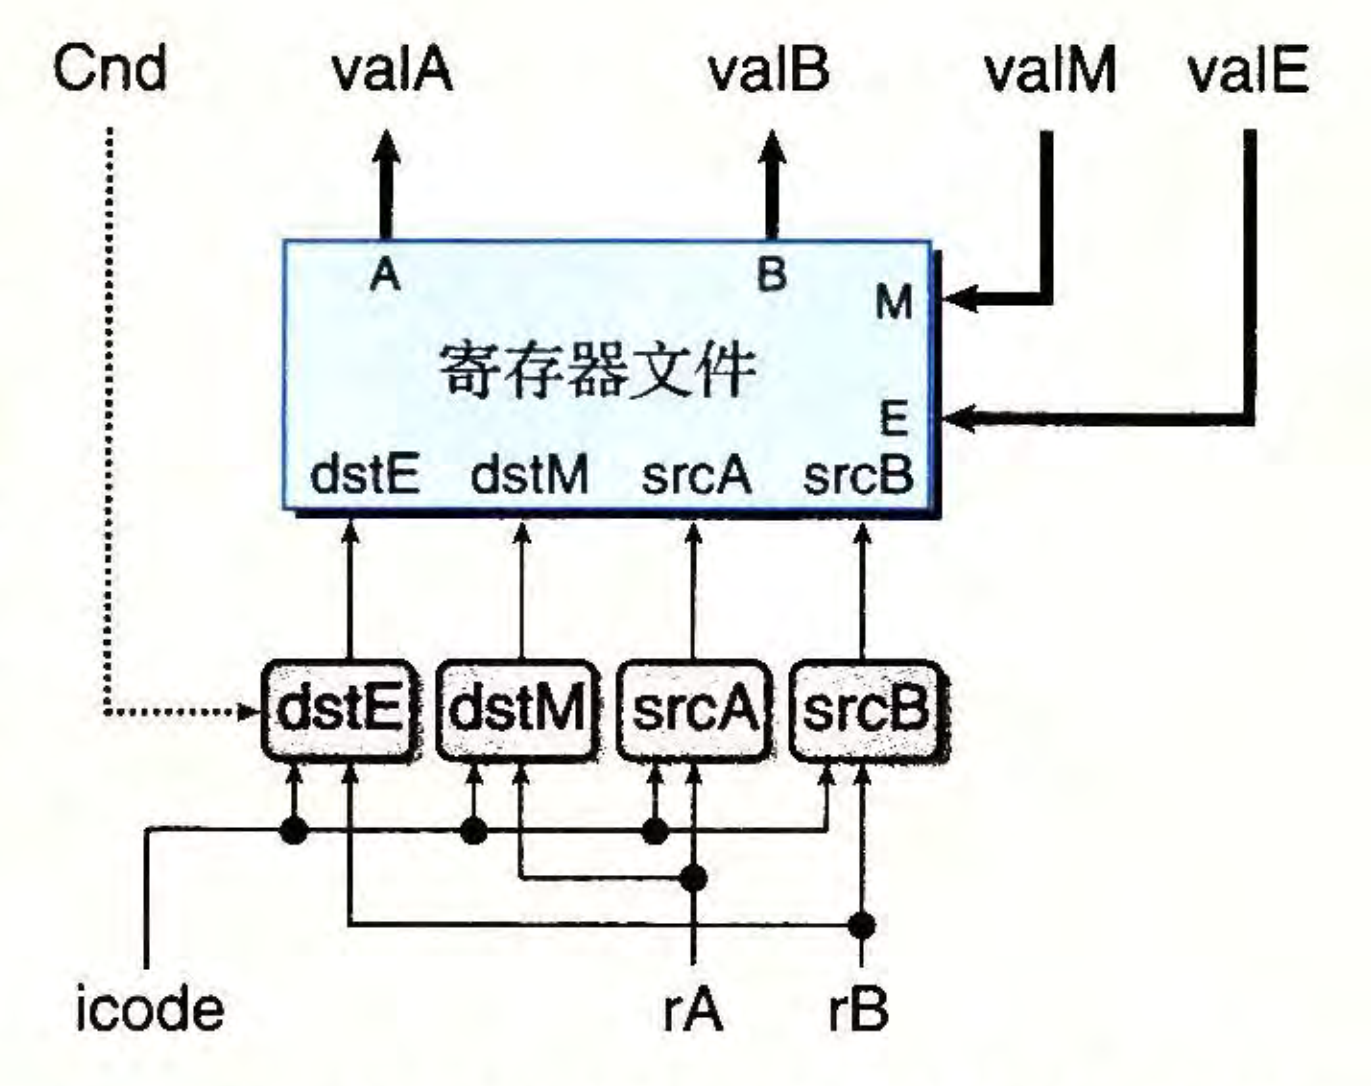
\includegraphics[width=0.5\textwidth]{decode.png}
\end{figure}

根据指令代码 icode 以及寄存器指示值 rA 和 rB ,可能还会根据执行阶段计算出的 Cnd 条件信号,产生出四个不同的寄存器文件的寄存器 ID 。
两个读端口的地址输人为 srcA 和 srcB ,两个写端口的地址输入为 dstE 和 dstM 。

\begin{lstlisting}[style=CStyle]
word srcA = [
    icode in { IRRMOVQ, IRMMOVQ, IOPQ, IPUSHQ } : rA;
    icode in { IPOPQ, IRET } : RRSP;
    1 : RNONE; # Don't need register
];
# WARNING: Conditional move not implemented correctly here
word dstE = [
    icode in { IRRMDVQ } : rB;
    icode in { IIRMOVQ, IOPQ } : rB;
    icode in { IPUSHQ, IPOPQ, ICALL, IRET } : RRSP;
    1 : RNONE; # Don't write any register
];
\end{lstlisting}

\subsubsection{执行阶段}

\begin{figure}[H]
    \centering
    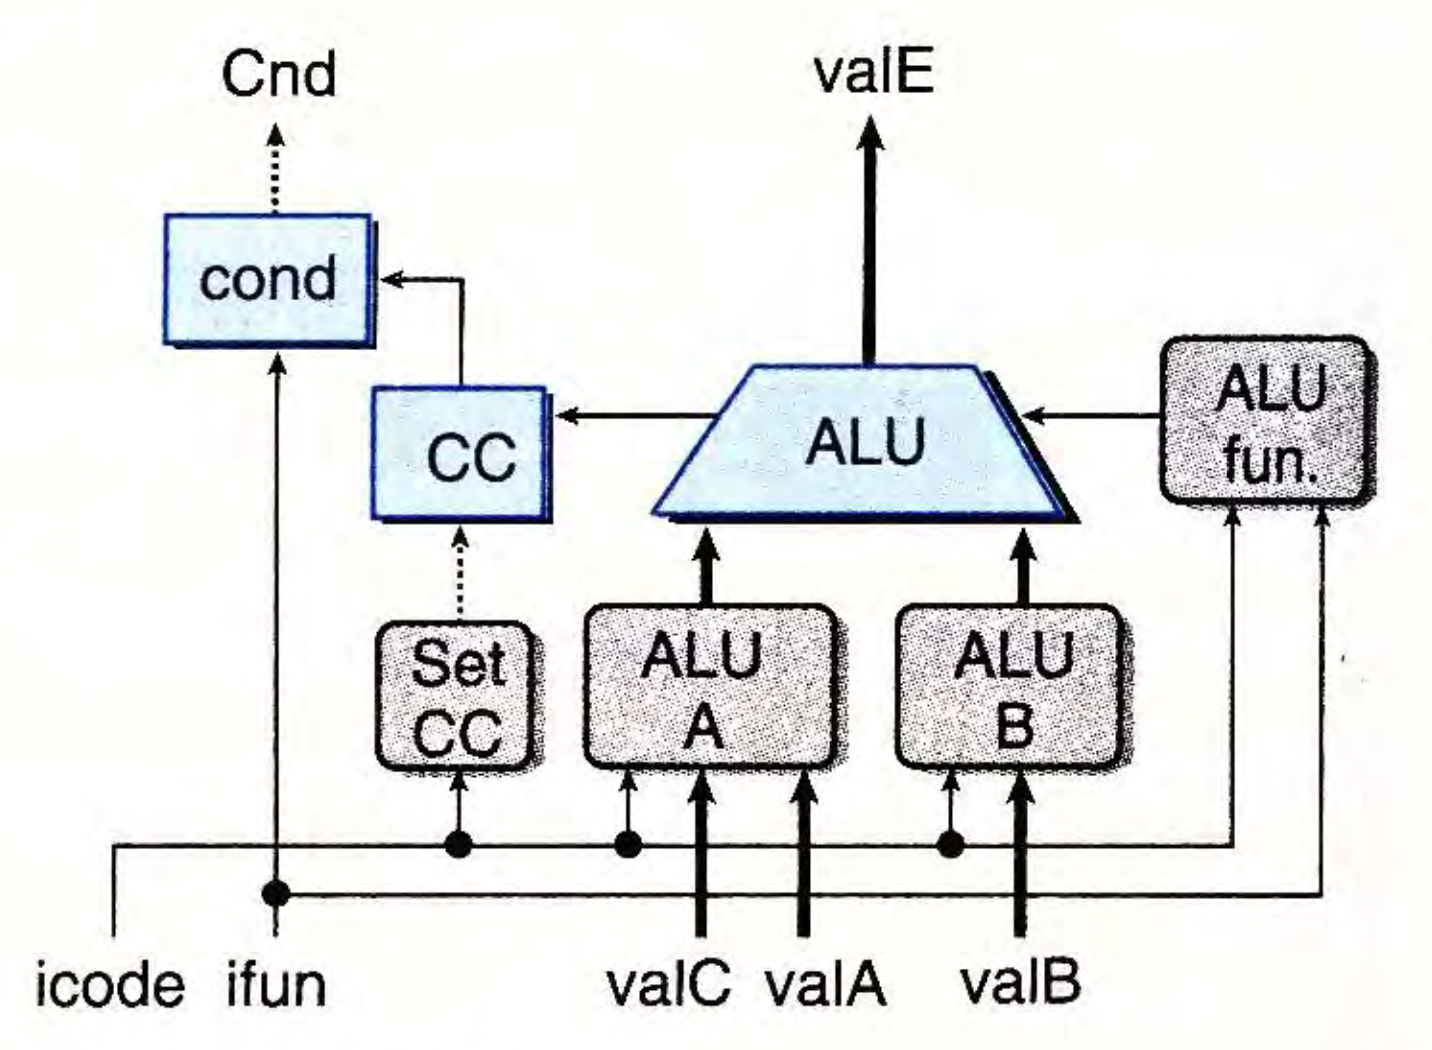
\includegraphics[width=0.5\textwidth]{execute.png}
\end{figure}

ALU 单元根据 alufun 信号的设置,对输入 aluA 和 aluB 执行 ADD 、 SUBTRACT 、 AND 或 EXCLUSIVEOR 运算,输出为 valE 信号。
\begin{lstlisting}[style=CStyle]
word aluA = [
    icode in { IRRMOVQ, IOPQ } : valA;
    icode in { IIRMOVQ, IRMMOVQ, IMRMOVQ } : valC;
    icode in { ICALL, IPUSHQ } : -8;
    icode in { IRET, IPOPQ } : 8;
    # Other instructions don't need ALU
];
word alufun = [
    icode == IDPQ : ifun;
    1 : ALUADD
];
\end{lstlisting}

执行阶段还包括条件码寄存器。
每次运行时, ALU 都会产生三个与条件码相关的信号零、符号和溢出。
不过,我们只希望在执行 OPq 指令时才设置条件码。
因此产生了一个信号 set cc 来控制是否该更新条件码寄存器。
\begin{lstlisting}[style=CStyle]
bool set_cc = icode in { IDPQ };
\end{lstlisting}

标号为 "cond" 的硬件单元会根据条件码和功能码来确定是否进行条件分支或者条件数据传送。
它产生信号 Cnd ,用于设置条件传送的 dstE ,也用在条件分支的下一个 PC 逻辑中。

\subsubsection{访存阶段}
\begin{figure}[H]
    \centering
    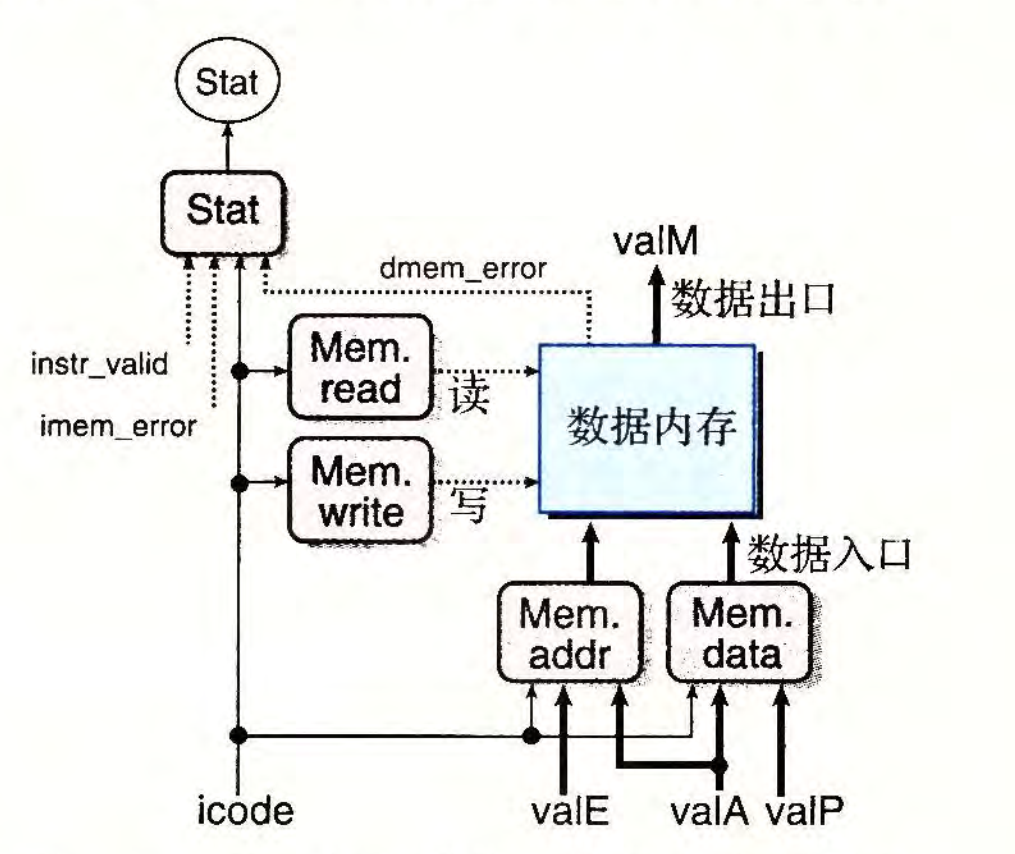
\includegraphics[width=0.5\textwidth]{memory.png}
\end{figure}

访存阶段的任务就是读或者写程序数据。两个控制块产生内存地址和内存输入数据的值。
另外两个块产生表明应该执行读操作还是写操作的控制信号。
当执行读操作时,数据内存产生值 valM 。
\begin{lstlisting}[style=CStyle]
word mem_addr = (
    icode in { IRMMOVQ , IPUSHQ, ICALL, IMRMOVQ } : valE;
    icode in { IPOPQ, IRET } : valA;
    # Other instructions don't need address
);
bool mem_read = icode in { IMRMOVQ, IPOPQ, IRET };
\end{lstlisting}

访存阶段最后的功能是根据取值阶段产生的 icode 、 imem error 、 instr valid 值
以及数据内存产生的 dmem error 信号,从指令执行的结果来计算状态码 Stat 。

\subsubsection{写回阶段}
\begin{figure}[H]
    \centering
    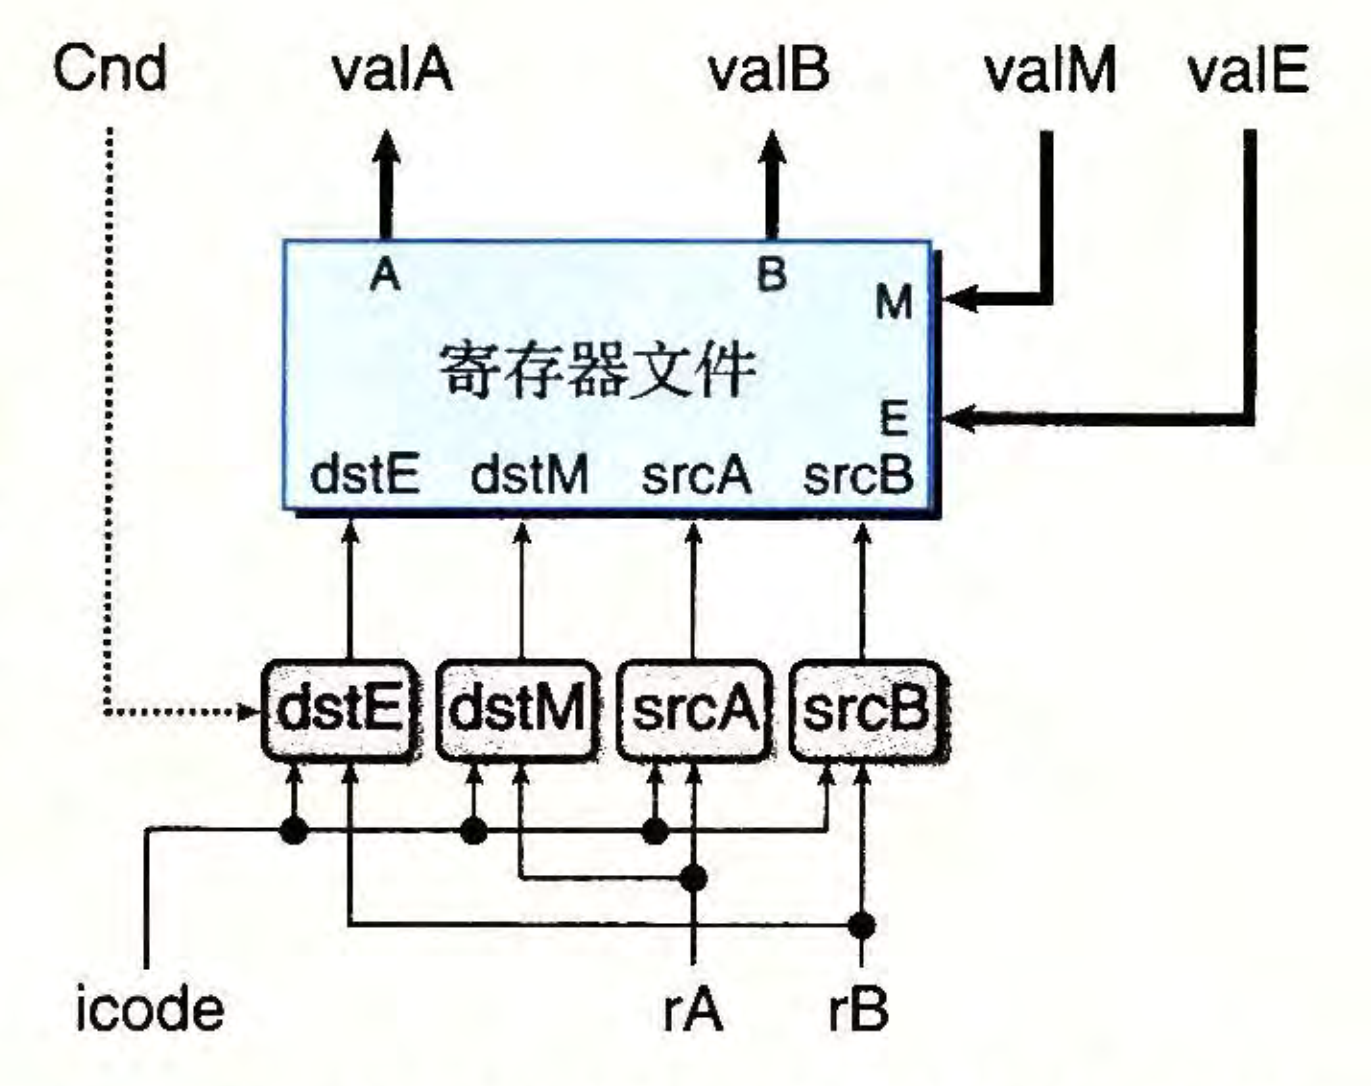
\includegraphics[width=0.5\textwidth]{write-back.png}
\end{figure}

写回阶段的任务是将执行阶段产生的值 valE 或者访存阶段产生的值 valM 写入寄存器文件。

\subsubsection{更新 PC 阶段}
\begin{figure}[H]
    \centering
    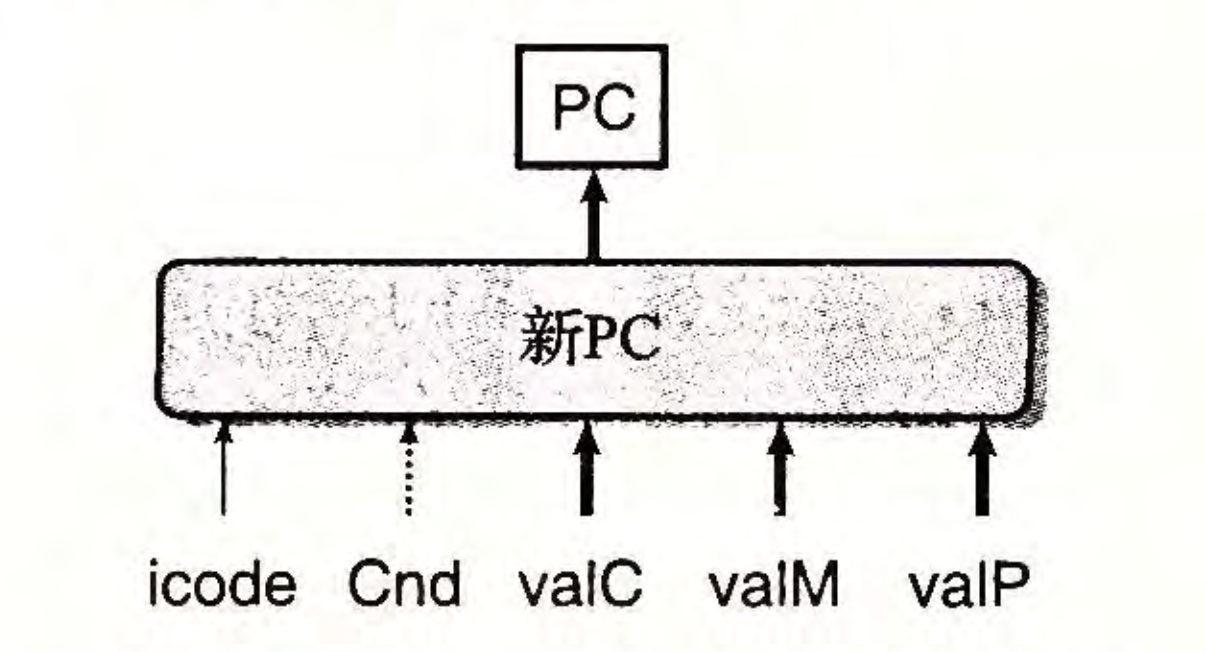
\includegraphics[width=0.5\textwidth]{PC-update.png}
\end{figure}

SEQ 中最后一个阶段会产生程序计数器的新值。
依据指令的类型和是否要选择分支,新的 PC 可能是 valC 、 valM 或 valP 。
\begin{lstlisting}[style=CStyle]
word new_pc = [
    # Call. Use instruction constant
    icode == ICALL : valC;
    # Taken branch. Use instruction constant
    icode == IJXX && Cnd : valC;
    # Completion of RET instruction. Use value from stack
    icode == IRET : valM;
    # Default: Use incremented PC
    1 : valP;
];
\end{lstlisting}

\subsubsection{SEQ 的时序}

SEQ 的实现包括组合逻辑和两种存储器设备:时钟寄存器(程序计数器和条件码寄存器),随机访问存储器(寄存器文件、指令内存和数据内存)。
组合逻辑不需要任何时序或控制,只要输入变化了,值就通过逻辑门网络传播。
存储器设备通过一个时钟信号来控制,它触发将新值装载到寄存器以及将值写到随机访问存储器中。

\begin{figure}[H]
    \centering
    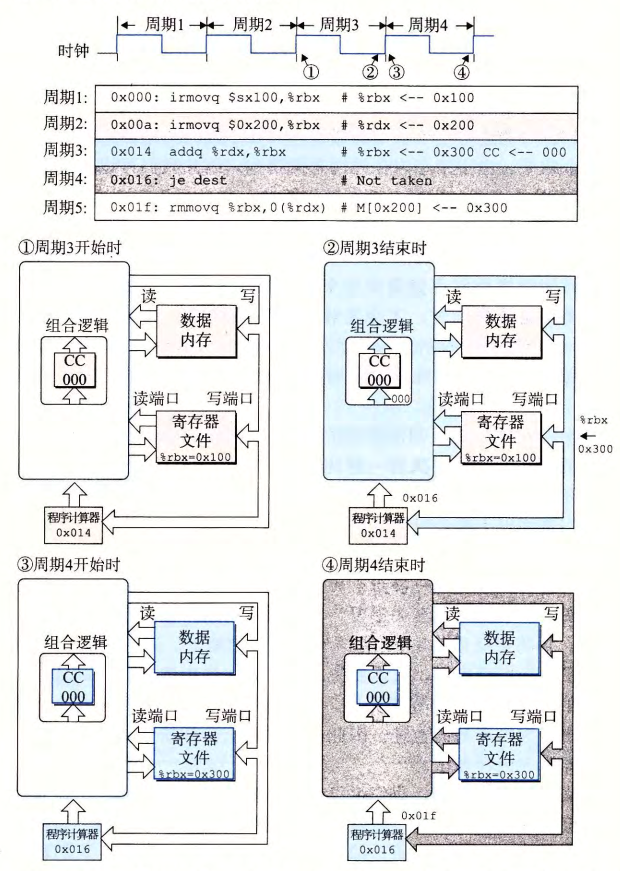
\includegraphics[width=0.8\textwidth]{SEQ-operation.png}
\end{figure}

\subsection{Y86-64 的流水线实现}

\subsubsection{PC 选择和取指阶段}
\paragraph{分支预测}
\paragraph{控制冒险}
\subsubsection{译码和写回阶段}
\paragraph{数据冒险}
\subsubsection{执行阶段}
\subsubsection{访存阶段}

\subsubsection{控制逻辑}
\paragraph{控制机制}
\paragraph{触发条件}
\paragraph{处理}
\paragraph{控制条件的组合}














\newpage